\documentclass[aps,prl,twocolumn,groupedaddress,showkeys]{revtex4}

\usepackage{graphicx}

\begin{document}

\title{Thin Film Deposition}
\author{309248035 \\
				D.G. Wilcox}

\noaffiliation{}

\date{\today}

\begin{abstract}
\end{abstract}

\keywords{supttering deposition, evaporation deposition}


\maketitle


\section{Introduction}

The aim of this experiment was to measure the conductivity of a thin film of copper wrt. thickness. The introduction deals with the concepts of evaporation and sputtering deposition techniques, as well as a technique for measuring thin film thickness. The procedure outlines how the required vacuum was obtained and conductivity was measured. The results are represented by a chart of Resistance Vs Thickness and is accompanied by some discussion, followed by conclusions.

\subsection{Thin Film Deposition Techniques}

Thin film deposition is a process that takes a source material and applies a thin film of it to a target substrate. The purposes are generally related to electronics, and involve thin films of conductors and the two techniques covered by this experiment are deposition via evaporation of the source material and deposition via sputtering of the source material.

\subsection{Evaporation Deposition}

The basic principle of Evaporation Deposition is to evaporate a metal (in this case aluminium) and allow it to condense on the target substrate. This forms an even coating of aluminium on the substrate. 

In more detail, the evaporation is done in a vacuum chamber. This is to avoid gas particles other than the aluminium being present and interfering with the process. The way the aluminium is boiled is by wrapping it around tungsten, which is then short circuited to provide heat. Since the melting point for tungsten is greater than the boiling point for aluminium, the tungsten is a suitable metal for the process.

\subsection{Sputtering Deposition}

Sputter deposition, rather then evaporating the source material, chips away from it causing the ejected particles to fall on the substrate material. This experiment used positively charged Argon ions from a plasma and accelerated them to the copper source, dislodging copper atoms and causing them to recondense on the substrate.


\subsection{Crystal Monitors}

In order to measure the thickness of the film while performing sputtering deposition a crystal monitor was used. A crystal monitor will measure the change in vibration frequency as it becomes more massive (due to the source material being deposited on its surface).


\section{Procedure}

\subsection{Preparation of the Substrate}

In order to perform evaporation deposition a vacuum of $1\times10^{-4}$ mbar was required. This was achieved by sequentially using a rotary pump and a diffusion pump.

Prior to evacuating the chamber the substrate (two glass microscope slides) was cleaned with alcohol and left on the floor of the chamber covered by a third slide as shown in figure~\ref{fig:slideArrangement}.

\begin{figure}[h]
	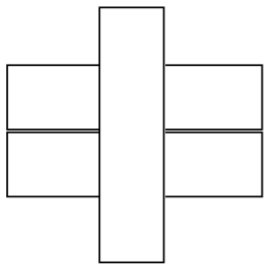
\includegraphics[width=0.6\linewidth]{glassSlideArrangement.png}
	\caption{Crossed glass slide arrangement}
	\label{fig:slideArrangement}
\end{figure}

Tungsten was wrapped in aluminium in the chamber in a way that we could provide about 30 A of current when short-ciruiting it.

Once everything was ready and in the chamber it was evacuated down to the required pressure. Once there the aluminium was evaporated until enough had condensed on the walls of the chamber to block light from passing through it. At this point the substrate was left to cool and then eventually removed.


\subsection{In-situ Conductivity Measurements}



\section{Results}

\subsection{Data}

\subsection{Discussion}

\section{Conclusions}

\section{Acknowledgments}

\end{document}
